\section{Designidee\cite{MaterialDesign}}

Die Grundidee hinter dem Design entspringt aus dem Wunsch eine moderne und intuitiv bedienbare Benutzeroberfläche zu bieten. Diese hat sowohl simpel als auch ansprechend und kreativ auszusehen.

Die größten Faktoren für Zufriedenheit der Nutzer ist die Gestaltung, Aufteilung und Präsentation einer Applikation. Deshalb wird sich an die Material Design Richtlinien gehalten. Laut Material Design ist die Designsprache eine Vereinigung aus klassischen Designprinzipien und den Möglichkeiten, welche durch Technische Innovationen geschaffen werden.
Die Einheitlichkeit des Designs ist ein ebenso wichtiger Aspekt. Das Nutzererlebnis soll Plattform, Gerät und Eingabemethode unabhängig gleich sein.
Unter allen diesen Vorgaben und Richtlinien ein Unikates und Ansprechendes Design zu entwerfen ist die Aufgabe, welche es umzusetzen gilt.


\section{Farben\cite{MaterialDesignColors}}
Gerade bei Webseiten, welche im Zusammenhang mit Essen stehen sind Farben wichtig. Die Farben bestimmen die Stimmung des Nutzers und bieten einen größeren Anreiz auf der Seite zu bleiben.

Die Farben sollen einen gewissen genießbaren Eindruck machen, deshalb wurden ausschließlich Farben verwendet welche in natürlichen Lebensmitteln Vorkommen.

Der Prozess lief folgendermaßen ab:
Es wurden sich Farben gefunden, welche laut Material Design zu einem Harmonischem Ganzen beitragen und genügend Kontrast bieten. Dann wurden diese durch Reverse-Lookup über Google.com in Bildern welche Tags wie „Essen“, „Tasty“ oder „Delicous“ hatten wiedergefunden. Die Bilder zeigen nun Lebensmittel welche ähnlichen Farben wie die Wunschfarben aufweisen. Nun wurden die Wunschfarben nur noch an eben genau diese Natürlichen Farben angepasst.

BILD
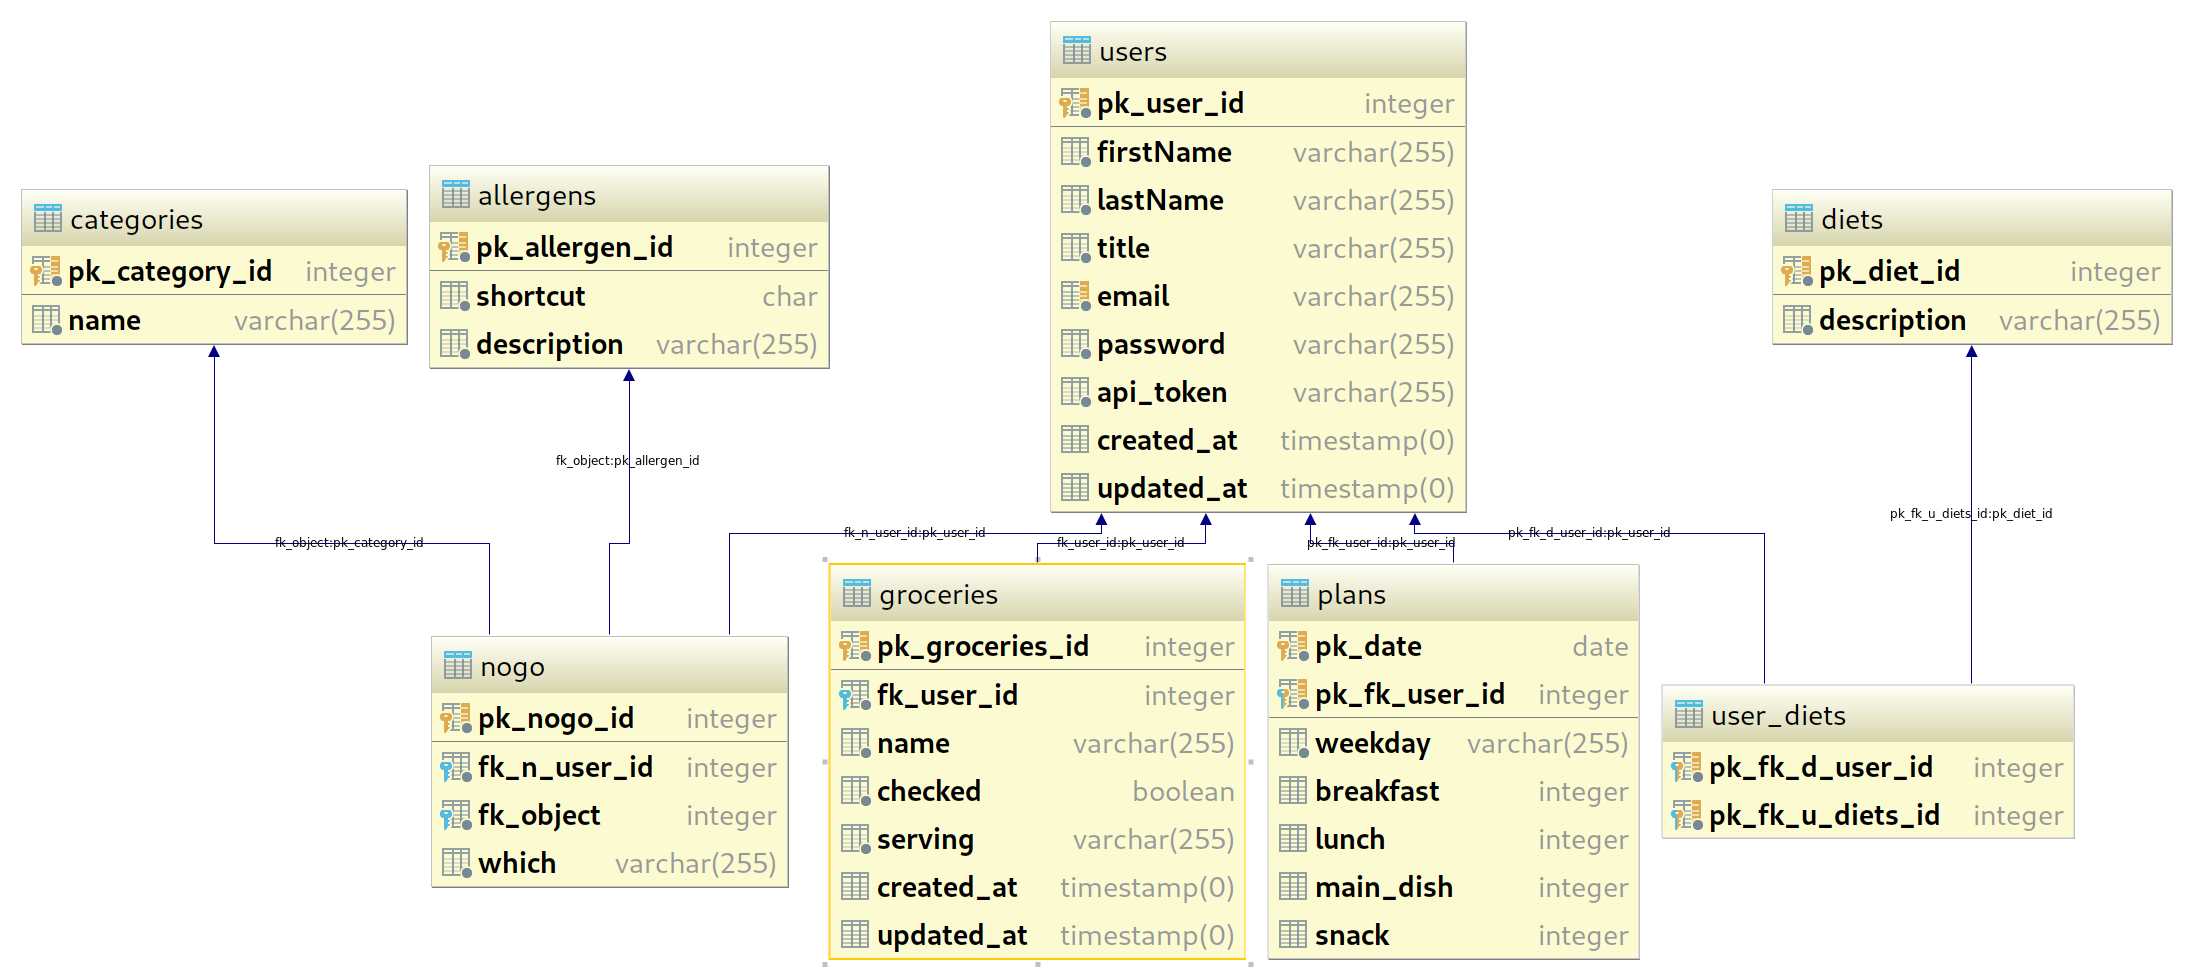
\includegraphics{threesixfive.png}


\section{Logo\cite{Logo}}
Das Logo ist der einfachste und direkteste Weg sich als Marke, Produkt oder Applikation Visuell auszudrücken. Es übermittelt die Grundidee der Applikation auf eine simple und dennoch aussagekräftige Art und Weise. Die für die Applikation konzipierte Designsprache ist in dem Logo erkennbar und reflektiert so die Identität der Applikation.


\subsection{Die Erstellung mittels Adobe Photoshop und Adobe Illustrator}
Das Logo sollte die Applikation repräsentieren und leicht mit Kochen und Rezepten in Verbindung gebracht werden können.

Mit der Umsetzung wurde begonnen indem auf Papier grobe Gedanken in Form von Skizzen aufgezeichnet wurden und so wurde mit diversen Ideen herumprobiert, um eine genauere Vorstellung zu bekommen. In diesem Prozess entstand die Idee einen Pfannenwender und Kochlöffel als Typische Symbole des Kochens zu verwenden.

Nun wurden der Pfannenwender und Kochlöffel in Photoshop mithilfe von groben Formen erstellt. Die beiden Symbole wurden überkreuzt um ein „Wappen“-ähnliches Aussehen zu erreichen. Der Entwurf wurde weiter verfeinert und angepasst. In diesem Prozess wurde das gesamte Team involviert sodass jedes Mitglied seine Gedanken preisgeben konnte. Nachdem es zu der Zufriedenheit aller verbessert wurde hat man den Entwurf zu Adobe Illustrator exportiert.

Adobe Illustrator bietet hervorragende Tools zur Erstellung von Vektorgrafiken. Letzte kleine Verbesserungen wie die exakte Positionierung wurde vorgenommen. Der Entwurf wurde in Illustrator nun vektorisiert indem er mit Pfaden nachgezogen wurde. Nach letzter Überprüfung wurde das fertige Logo exportiert. Hierzu wurden diverse Formate abgespeichert.

\begin{table}[]
\begin{tabular}{|l|l|l|}
\hline
\multicolumn{1}{|c|}{\textbf{Name}} & \multicolumn{1}{c|}{\textbf{Dateiendung}} & \multicolumn{1}{c|}{\textbf{Verwendung}}                                                                                                                                           \\ \hline
Adobe Illustrator                   & .ai                                       & \begin{tabular}[c]{@{}l@{}}Das Original File für spätere \\ Editierungen.\end{tabular}                                                                                             \\ \hline
Portable Document Format            & .pdf                                      & \begin{tabular}[c]{@{}l@{}}Zur Verbreitung / Teilung des \\ Logos. Universell verwendbar \\ auf nahezu allen Geräten. Hier \\ wird eine Vektordatei \\ abgespeichert.\end{tabular} \\ \hline
Portable Network Graphic            & .png                                      & \begin{tabular}[c]{@{}l@{}}Pixelgrafikformat welches\\ Transparenz erlaubt. Zur\\ Verwendung an Desktop\\ Computern und bei der\\ Digitalen Bildbearbeitung.\end{tabular}          \\ \hline
Scalable Vector Graphic             & .svg                                      & \begin{tabular}[c]{@{}l@{}}Vektordatei zur Verwendung\\ auf Webseiten. Verlustfrei\\ skalierbar.\end{tabular}                                                                      \\ \hline
\end{tabular}
\end{table}


\section{Angular Frontend\cite{AngularFrontend}}
Angular ist ein Framework, um interaktive Komponenten für eine Webseite zu erstellen. Es wurde als umfangreiches JavaScript Framework von der Google LLC entwickelt. Angular ist Open-Source-Software und ist eines der größten Front-End-Webapplikationsframeworks. Es ist in TypeScript geschrieben und aufgrund der eindeutigen Unterteilung der einzelnen Komponenten eignet es sich perfekt für ThreeSixFive.

Angular basiert auf der Model-View-Controller Art Code zu schreiben. Entwickler haben dieses Modell seit langem verwendet jedoch ist Angular das erste JavaScript Framework, welches darauf aufbaut.

Dieses Prinzip teilt die Entwicklung auf drei Ebenen auf.

„View/Template“ als das sichtbare welches die Userexperience ausmacht und mit HTML und CSS/SCSS geschrieben wird.

„ViewModel/Component“ jede Komponente definiert eine Klasse, welche die Applikations-Daten und -Logik für ein Template enthalten.

„Service/Injector“ für Daten und Logik, welche keinem speziellem Template zugeordnet sind und welche man Komponenten-übergreifend verwenden möchte. Diese müssen mittels Injektor den Komponenten als Dependency übergeben werden.

Das Model-View-Controller Modell erlaubt die Wiederverwendung von Templates und Komponenten und ist somit ideal für die Applikation ThreeSixFive. Außerdem erlaubt das two-way data binding zwischen Template und Component ständige Updates zwischen beiden Ebenen. Ohne Angular müsste der Entwickler selbst sich um den ständigen Austausch zwischen Nutzer Eingaben und Aktion/Werte-Veränderungen in der Logik kümmern. Solch eine push und pull Logik selbst zu schreiben ist umständlich und fehleranfällig.

Im Folgenden Diagram wird aufgezeigt wie Angular mit dem DOM kommuniziert.
Es werden vier verschiedene Formen des data-bindings gezeigt. Jede Form hat eine Richtung:
\begin{itemize}
\item Zu dem DOM
\item Vom DOM
\item Beidseitig sowohl vom DOM als auf zum DOM
\end{itemize}

Angular modifiziert direkt die DOM-Struktur einer Seite und fügt sich nicht in das HTML ein. Dies führt zu einer besseren Performance der Applikation.

In dieser Umgebung, welche von Angular geboten wird, gilt es nun unsere Applikation umzusetzen.
